% -*- coding: utf-8 -*-

\begin{chapter}{Завихренность в океане}\label{chap:12}
% \chapter{Vorticity in the Ocean} 
Большинство потоков жидкостей, с которыми мы знакомы, в ваннах и в
плавательных бассейнах, не являются вращательными, или их вращение
настолько слабо, что оно не представляет интерес, за исключением может
быть того случая, когда происходит слив воды в ванной. В результате у
нас нету хорошего интуитивного понимания вращательного потока. В
океане вращение и сохранение завихренности сильно влияет на потом на
расстояниях, превышающих несколько десятков километров. Последствие
вращения приводит к результатам, которых не видно в нашей повседневной
практике с течениями. Например, спросите себя~--- почему
завихренность напряжения трения ветра приводит к тому, что транспорт
масс происходит в северо-южном направлении а не в востоко-западном?
Что особенного в северо-южном переносе? В этой главе мы исследуем
некоторые последствия вращения для потоков в океане.
%
% Most of the fluid flows with which we are familiar, from bathtubs to
% swimming pools, are not rotating, or they are rotating so slowly that
% rotation is not important except maybe at the drain of a bathtub as
% water is let out. As a result, we do not have a good intuitive
% understanding of rotating flows. In the ocean, rotation and the
% conservation of vorticity strongly influence flow over distances
% exceeding a few tens of kilometers. The consequences of the rotation
% leads to results we have not seen before in our day-to-day dealings
% with fluids.  For example, did you ask yourself why the curl of the
% wind stress\index{wind stress!curl of} leads to a mass
% transport\index{transport!mass} in the north-south direction and not
% in the east-west direction? What is special about north-south motion?
% In this chapter, I will explore some of the consequences of rotation
% for flow in the ocean.

\begin{section}{Определение Завихренности}
% \section{Definitions of Vorticity}
Если говорить простыми словами, завихренность~--- это вращение
потока. Скорость вращения можно определить разными путями. Рассмотрим
резервуар с водой, стоящий на столе в лаборатории. Вода может
вращаться в резервуаре. В добавок ко вращению воды, вращаются
резервуар и лаборатория, поскольку они находятся на поверхности
вращающейся планеты. Эти два процесса различны и приводят к двум типам
завихренности.
%
% In simple words, vorticity\index{vorticity} is the rotation of the
% fluid. The rate of rotation can be defined various ways. Consider a
% bowl of water sitting on a table in a laboratory. The water may be
% spinning in the bowl. In addition to the spinning of the water, the
% bowl and the laboratory are rotating because they are on a rotating
% earth. The two processes are separate and lead to two types of
% vorticity.

\begin{paragraph}{Планетарная завихренность.}
% \paragraph{Planetary Vorticity}
Все, что находится на Земле, включая океаны, атмосферу и резервуары с
водой, вращается вместе с Землей. Это вращение называется планетарной
завихренностью и обозначается символом~$f$. Она равна удвоенной скорости
вращения Земли в конкретной точке.
\begin{equation}
\boxed{f \equiv 2\,\Omega \sin \varphi \,\, \text{(radians/s)} 
  = 2 \sin \varphi \,\, \text{(cycles/day)}}
\end{equation}
Планетарная завихренность~--- это параметр Кориолиса, который мы
использовали ранее при обсуждении океанических потоков. Этот параметр
достигает максимального значения на полюсах, где он равен удвоенной
скорости вращения Земли. Заметим что завихренность равна нулю на
экваторе и отрицательна в южном полушарии (поскольку угол~$\varphi$
отрицателен).
%
% Everything on earth, including the ocean, the atmosphere, and bowls of
% water, rotates with the earth. This rotation is the \textit{planetary
% vorticity}\index{planetary vorticity|textbf} $f$. It is twice the
% local rate of rotation of earth:
% \begin{equation}
% \boxed{f \equiv 2\,\Omega \sin \varphi \,\, \text{(radians/s)} 
%   = 2 \sin \varphi \,\, \text{(cycles/day)}}
% \end{equation}
% Planetary vorticity is the Coriolis parameter\index{Coriolis parameter} 
% I used earlier to discuss flow in the ocean. It is greatest
% at the poles where it is twice the rotation rate of earth. Note that
% the vorticity vanishes at the equator and that the vorticity in the
% southern hemisphere is negative because $\varphi$ is negative.
\end{paragraph}

\begin{paragraph}{Относительная завихренность.}
% \paragraph{Relative Vorticity}
Океан и атмосфера вращаются со скоростью, которая не равна в точности
той скорости вращения, которую имеет планета. Они (океан и атмосфера)
имеют некоторое вращение относительно Земли благодаря течениям и
ветрам. Относительная завихренность~$\zeta$ это та завихренность, которая
возникает вследствии течений в океане. Математически ее можно выразить
так:
\begin{equation}
\boxed{ \zeta \equiv \text{curl}_z\, \textbf{V} =
\frac{\partial{v}}{\partial{x}}-\frac{\partial{u}}{\partial{y}} }
\end{equation}
Где $\textbf{V} = (u, v)$ вектор горизонтальной скорости. Мы
предполагаем что поток двумерный. Это допущение истинно если
протяженность потока превышает расстояние несколько десятков
километров. $\zeta $~--- вертикальная компонента трехмерного вектора
завихренности~$\omega$, и иногда он обозначается как~$\omega{_z}$.
$\zeta$~положительный для вращения против часовой стрелки если
смотреть сверху. Тот же знак имеет вращение Земли в северном
полушарии.
%
% The ocean and atmosphere do not rotate at exactly the same rate as
% earth. They have some rotation relative to earth due to currents and
% winds. \textit{Relative vorticity}\index{relative vorticity|textbf}
% $\zeta$ is the vorticity due to currents in the ocean. Mathematically
% it is:
% \begin{equation}
% \boxed{ \zeta \equiv \text{curl}_z\, \textbf{V} =
% \frac{\partial{v}}{\partial{x}}-\frac{\partial{u}}{\partial{y}} }
% \end{equation}
% where $\textbf{V} = (u, v)$ is the horizontal velocity vector, and
% where we have assumed that the flow is two-dimensional. This is true
% if the flow extends over distances greater than a few tens of
% kilometers. $\zeta $ is the vertical component of the
% three-dimensional vorticity vector $\omega$, and it is sometimes
% written $\omega{_z}$. $\zeta$ is positive for counter-clockwise
% rotation viewed from above. This is the same sense as earth's rotation
% in the northern hemisphere.

\emph{Замечание об используемых обозначениях.} Символы, обычно
используемые в каком либо разделе океанографии, имеют совсем другое
значение в другом разделе. В этом разделе мы используем символ~$\zeta$
для обозначения завихренности, но в главе 10 мы используем~$\zeta$ для
обозначения высоты поверхности моря. Мы можем использовать
обозначение~$\omega_z$ для относительной завихренности, но
символ~$\omega$ так же широко применяется для обозначения частоты
вращения в радианах в секунду. Я сделал попытку исключить большинство
сбивающих с толку случаев, но двойное использование
символа~$\zeta$~--- единственный случай, с которым нам придется
мириться. К счастью он не должен вызывать большую путаницу.
%
% \textit{Note on Symbols} Symbols commonly used in one part of
% oceanography often have very different meaning in another part. Here I
% use $\zeta$ for vorticity, but in Chapter 10, I used $\zeta$ to mean
% the height of the sea surface. I could use $\omega_z$ for relative
% vorticity, but $\omega$ is also commonly used to mean frequency in
% radians per second. I have tried to eliminate most confusing uses, but
% the dual use of $\zeta$ is one we will have to live with. Fortunately,
% it shouldn't cause much confusion.

Для жесткого тела, вращающегося со скоростью~$\Omega$, curl\textbf{V}
$= 2\,\Omega$. Конечно потоку не нужно вращаться как жесткому телу что
бы иметь относительную завихренность. Завихренность может быть так же
результатом сдвига. Например, на северо/юго-западной границе в океане,
$u=0$, $v=v(x)$ и~$\zeta = \partial{v(x)}/\partial{x}$.
%
% For a rigid body rotating at rate $\Omega$, curl\textbf{V} $=
% 2\,\Omega$. Of course, the flow does not need to rotate as a rigid
% body to have relative vorticity. Vorticity can also result from
% shear. For example, at a north/south western boundary in the ocean,
% $u=0$, $v=v(x)$ and $\zeta = \partial{v(x)}/\partial{x}$.

$\zeta$ обычно намного меньше чем~$f$, и достигает максимального
значения на границе быстрых течений, таких как Гольфстрим. Что бы
получить представление о величине~$\zeta$, рассмотрим край Гольфстрима на
удалении от мыса Гатерас, где уменьшение скорости течения составляет 1
м/сек на 100 км на границе. Вихрь течения приблизительно равен (1
м/сек) / (100 км) = 0.14 оборот/сутки = 1 оборот/неделя. Следовательно
даже такое большое значения относительной завихренности почти в семь
раз меньше значения~$f$. Наиболее типичное значение относительной
завихренности, например завихренность в вихрях, равно одному обороту в
месяц.
%
% $\zeta$ is usually much smaller than $f$, and it is greatest at the
% edge of fast currents such as the Gulf Stream\index{Gulf
% Stream!vorticity}. To obtain some understanding of the size of
% $\zeta$, consider the edge of the Gulf Stream off Cape Hatteras where
% the velocity decreases by 1 m/s in 100 km at the boundary. The curl of
% the current is approximately (1 m/s)/(100 km) = 0.14 cycles/day = 1
% cycle/week. Hence even this large relative vorticity is still almost
% seven times smaller than $f$. A more typical values of relative
% vorticity, such as the vorticity of eddies, is a cycle per month.
\end{paragraph}

\begin{paragraph}{Абсолютная завихренность.}
% \paragraph{Absolute Vorticity}
Сумма планетарной и относительной завихренности называется абсолютной
завихренностью.
\begin{equation}
\boxed{ \text{Absolute Vorticity} \equiv (\zeta + f) }
\end{equation}
%
% \index{absolute vorticity}\index{vorticity!absolute}
% The sum of the planetary and relative vorticity is called
% \textit{absolute vorticity}\index{absolute vorticity|textbf}:
% \begin{equation}
% \boxed{ \text{Absolute Vorticity} \equiv (\zeta + f) }
% \end{equation}

Мы можем получить уравнения абсолютной завихренности в океане путем
простейших преобразований уравнений движения для потока невязкой
жидкости. Возьмем следующую систему уравнений:
\begin{subequations}
\begin{align}
 \frac{Du}{Dt} -f\,v &= -\frac{1}{\rho}\,\frac{\partial{p}}{\partial{x}} \\
 \frac{Dv}{Dt} +f\,u &= -\frac{1}{\rho}\,\frac{\partial{p}}{\partial{y}}
\end{align}
\end{subequations}
Если мы разложим общую производную, продифференцируем уравнение(12.4а)
по~$у$, а уравнение (12.4b) по~$х$ и вычтем первое из второго исключая при
этом слагаемые с давлением, то получим после некоторых алгебраических
преобразований следующее:
\begin{equation}
\boxed{ \frac{D}{Dt}\left(\zeta +f  \right) + \left(\zeta +f  \right)
\left(\frac{\partial{u}}{\partial{x}} +
\frac{\partial{v}}{\partial{y}} \right) = 0 }
\end{equation}
При выводе (12.15) мы использовали следующее:
\begin{equation}
\frac{Df}{Dt} = \frac{\partial{f}}{\partial{t}}
+u\,\frac{\partial{f}}{\partial{x}} +v\,\frac{\partial{f}}{\partial{y}} = \beta
\,v \notag
\end{equation}
Поскольку $f$ не зависит от времени и от долготы.
%
% We can obtain an equation for absolute vorticity in the ocean by
% manipulating the equations of motion for frictionless flow. We begin
% with:
% \begin{subequations}
% \begin{align}
% \frac{Du}{Dt} -f\,v &= -\frac{1}{\rho}\,\frac{\partial{p}}{\partial{x}} \\
% \frac{Dv}{Dt} +f\,u &= -\frac{1}{\rho}\,\frac{\partial{p}}{\partial{y}}
% \end{align}
% \end{subequations}
% If we expand the substantial derivative, and if we subtract
% $\partial\:/\partial{y}$ of (12.4a) from $\partial\:/\partial{x}$ of
% (12.4b) to eliminate the pressure terms, we obtain after some
% algebraic manipulations:
% \begin{equation}
% \boxed{ \frac{D}{Dt}\left(\zeta +f  \right) + \left(\zeta +f  \right)
% \left(\frac{\partial{u}}{\partial{x}} +
% \frac{\partial{v}}{\partial{y}} \right) = 0 }
% \end{equation}
% In deriving (12.5) we used:
% \begin{equation}
% \frac{Df}{Dt} = \frac{\partial{f}}{\partial{t}}
% +u\,\frac{\partial{f}}{\partial{x}} +v\,\frac{\partial{f}}{\partial{y}} = \beta
% \,v \notag
% \end{equation}
% because $f$ is independent of time $t$ and eastward distance $x$.
\end{paragraph}

\begin{paragraph}{Потенциальная завихренность.}
% \paragraph{Potential Vorticity}
Скорость вращения столба жидкости меняется если столб удлиняется или
укорачивается. Это изменяет завихренность через изменения
относительной завихренности $\zeta$. Что бы увидеть как это происходит
рассмотрим баротропный, геострофический поток в океане с глубиной
$H(x, y, t)$, где $H$~--- расстояние между поверхностью моря и
глубиной. Таким образом мы допускаем что поверхность имеет топографию
(рисунок 12.1).
%
% The rotation rate of a column of fluid changes as the column is
% expanded or contracted. This changes the vorticity through changes in
% $\zeta$. To see how this happens, consider barotropic,
% geostrophic\index{geostrophic currents!vorticity} flow in an ocean
% with depth $H(x, y, t)$, where $H$ is the distance from the sea
% surface to the bottom. That is, we allow the surface to have
% topography (figure 12.1).

\begin{figure}[t!]
\begin{center}
\makebox[120mm] [c]{\includegraphics{pics/vorticitysketch}}
\end{center}
\caption{Схема потока жидкости, использующаяся для вывода сохранения
потенциальной завихренности}
%% добавить отсылку к источнику (см. ниже)
\label{fig:vorticitysketch}
\vspace{-3ex}
\end{figure}
%
% \begin{figure}[t!]
% \centering
% \makebox[120mm] [c]{\includegraphics{vorticitysketch}}
% \footnotesize
% Figure 12.1 Sketch of fluid flow used \rule{0mm}{3ex}for deriving
% conservation of\\potential vorticity. After Cushman-Roisin (1994: 55).
%
% \label{fig:vorticitysketch}
% \vspace{-3ex}
% \end{figure}

Интегрирование уравнения неразрывности (7.19) от дна до поверхности
океана дает следующее (Cushman-Roisin, 1994):
\begin{equation}
\left( \frac{\partial{u}}{\partial{x}} + \frac{\partial{v}}{\partial{y}}\right) \int_{b}^{b+H} dz + w \bigr|_{b}^{b+H} = 0
\end{equation}
Где $b$~--- топография глубины, $H$~--- толщина водного
столба. Граничные условия требуют что бы поток на поверхности и дна
был вдоль поверхности и дна. Таким образом вертикальная компонента
скорости на поверхности и дне равна:
\begin{align}
w(b+H) &= \frac{\partial{(b+H)}}{\partial{t}} 
          + u\,\frac{\partial{(b+H)}}{\partial{x}}
          + v\, \frac{\partial{(b+H)}}{\partial{y}} \\
w(b)   &= u\,\frac{\partial{(b)}}{\partial{x}}
          + v\,\frac{\partial{(b)}}{\partial{y}}
\end{align}
Подставляя (12.7) и (12.8) в (12.6) мы получим:
\begin{displaymath}
 \left( \frac{\partial{u}}{\partial{x}} 
     + \frac{\partial{v}}{\partial{y}}\right) + \frac{1}{H}\,\frac{DH}{Dt} = 0
\end{displaymath}
Подстановка этого в (12.5) дает:
\begin{displaymath}
\frac{D}{Dt}\left(\zeta +f  \right) -\frac{\left(\zeta +f
\right)}{H}\,\frac{DH}{Dt} = 0
\end{displaymath}
Которое может быть написано в виде:
\begin{displaymath}
\frac{D }{Dt}\,\left( \frac{\zeta + f}{H} \right) = 0
\end{displaymath}
Величина в круглых скобках должна быть константой. Эта величина носит
название~--- потенциальная завихренность~$\Pi$. Потенциальная
завихренность сохраняется вдоль траектории потока.
\begin{equation}
\boxed{\text{Potential Vorticity} = \Pi \equiv \frac{\zeta + f}{H} }
\end{equation}
%
% Integrating the continuity equation (7.19) from the bottom to the top
% of the ocean gives (Cushman-Roisin, 1994):
% \begin{equation}
% \left( \frac{\partial{u}}{\partial{x}} + \frac{\partial{v}}{\partial{y}}\right) \int_{b}^{b+H} dz + w \bigr|_{b}^{b+H} = 0
% \end{equation}
% where $b$ is the topography of the bottom, and $H$ is the depth of the
% water. Notice that $\partial{u}/\partial{x}$ and
% $\partial{v}/\partial{y}$ are independent of $z$ because they are
% barotropic, and the terms can be taken outside the integral.
%
% The boundary conditions require that flow at the surface and the
% bottom be along the surface and the bottom. Thus the vertical
% velocities at the top and the bottom are:
% \begin{align}
% w(b+H) &= \frac{\partial{(b+H)}}{\partial{t}} + u\,\frac{\partial{(b+H)}}{\partial{x}}+v\, \frac{\partial{(b+H)}}{\partial{y}} \\
% w(b) &= u\,\frac{\partial{(b)}}{\partial{x}}+v\,\frac{\partial{(b)}}{\partial{y}}
% \end{align}
% where we used $\partial{b}/\partial{t} = 0$ because the bottom does
% not move, and $\partial{H}/\partial{z} = 0$. Substituting (12.7) and
% (12.8) into (12.6) we obtain
% \begin{displaymath}
% \left( \frac{\partial{u}}{\partial{x}} + \frac{\partial{v}}{\partial{y}}\right) + \frac{1}{H}\,\frac{DH}{Dt} = 0
% \end{displaymath}
% Substituting this into (12.5) gives:
% \begin{displaymath}
% \frac{D}{Dt}\left(\zeta +f  \right) -\frac{\left(\zeta +f
% \right)}{H}\,\frac{DH}{Dt} = 0
% \end{displaymath}
% which can be written:
% \begin{displaymath}
% \frac{D }{Dt}\,\left( \frac{\zeta + f}{H} \right) = 0
% \end{displaymath}
% The quantity within the parentheses must be constant. It is called
% \textit{potential vorticity}\index{potential vorticity|textbf}
% $\Pi$. Potential vorticity is conserved along a fluid trajectory:
% \begin{equation}
% \boxed{\text{Potential Vorticity} = \Pi \equiv \frac{\zeta + f}{H} }
% \end{equation}

Для бароклинного потока в постоянно стратифицированном потоке,
потенциальная завихренность может быть выражена:
\begin{equation}
 \Pi = \frac{\zeta + f}{\rho} \cdot \nabla \lambda
\end{equation}
Где $\lambda$~--- любая сохраняющаяся величина для каждого элемента
потока. В частности, если~$\lambda = \rho$, тогда:
\begin{equation}
 \Pi = \frac{\zeta + f}{\rho}\,\frac{\partial{\rho}}{\partial{z}}
\end{equation}
Если, горизонтальные градиенты плотности малы, по сравнению с
вертикальными градиентами, то (12.11) будет хорошим приближением для
термоклина. В водной толще большинства районов океана,$f \gg \zeta$ 
и (12.11) может быть выражена в виде:
\begin{equation}
 \Pi = \frac{f}{\rho}\,\frac{\partial{\rho}}{\partial{z}}
\end{equation}
Это соотношение позволяет определить потенциальную завихренность в
различных слоях водной толщи океана напрямую из гидрографических
данных не привлекая информацию о поле скоростей.
%
% For baroclinic flow in a continuously stratified fluid, the potential
% vorticity can be written (Pedlosky, 1987: \S 2.5):
% \begin{equation}
% \Pi = \frac{\zeta + f}{\rho} \cdot \nabla \lambda
% \end{equation}
% where $\lambda$ is any conserved quantity for each fluid element. In,
% particular, if $\lambda = \rho$ then:
% \begin{equation}
% \Pi = \frac{\zeta + f}{\rho}\,\frac{\partial{\rho}}{\partial{z}}
% \end{equation}
% assuming the horizontal gradients of density are small compared with
% the vertical gradients, a good assumption in the
% thermocline\index{thermocline}. In most of the interior of the ocean,
% $f \gg \zeta$ and (12.11) is written (Pedlosky, 1996, eq 3.11.2):
% \begin{equation}
% \Pi = \frac{f}{\rho}\,\frac{\partial{\rho}}{\partial{z}}
% \end{equation}
% This allows the potential vorticity of various layers of the ocean to
% be determined directly from hydrographic data\index{hydrographic
% data!and potential vorticity} without knowledge of the velocity field.
\end{paragraph}
\end{section}

\begin{section}{Сохранение завихренности}
% \section{Conservation of Vorticity}
Угловой момент любого изолированного вращающегося тела
сохраняется. Вращающееся тело может быть вихрем в океане или планетой
в пространстве. Если вращающееся тело не изолировано, тогда, в случае
если оно связано с другим телом, возможен перенос углового момента
между телами. При этом не нужно что бы был физический контакт между
двумя телами. Гравитационные силы могут переносить момент между телами
в пространстве. Мы еще вернемся к этой теме в главе 17 когда будем
обсуждать приливы в океане. В этой же разберем сохранение
завихренности во вращающемся океане.
%
% \index{vorticity!conservation of}The angular momentum of any isolated
% spinning body is conserved. The spinning body can be an eddy in the
% ocean or the earth in space. If the the spinning body is not isolated,
% that is, if it is linked to another body, then angular momentum can be
% transferred between the bodies. The two bodies need not be in physical
% contact. Gravitational forces can transfer momentum between bodies in
% space.  I will return to this topic in Chapter 17 when I discuss tides
% in the ocean. Here, let's look at conservation of vorticity in a
% spinning ocean.

Трение играет важную роль при передаче количества движения в
потоке. Трение передает количество движения от атмосферы к океану
через тонкий, вязкостный слой Экмана на поверхности моря. Трение
передает количество движения от океана к твердой земле через слой
Экмана на дне моря. Трение вдоль краев подводных гор приводит к
разнице давления на каждом крае гор, которое вызывает другой тип
сопротивления, т.н. сопротивление формы. Это тоже самое сопротивление,
которое вызывает сила ветра на машину, которая едет с высокой
скоростью. Тем не менее во всех обширных внутренних районах океана
поток свободный от трения и завихренность сохраняется. Такой поток
называют консервативным.
%
% Friction is essential for the transfer of momentum in a
% fluid. Friction transfers momentum from the atmosphere to the ocean
% through the thin, frictional, Ekman layer at the sea
% surface\index{Ekman layer}. Friction transfers momentum from the ocean
% to the solid earth through the Ekman layer at the sea floor. Friction
% along the sides of sub-sea mountains leads to pressure differences on
% either side of the mountain which causes another kind of drag called
% \textit{form drag}\index{form
% drag|textbf}\index{drag!form|textbf}. This is the same drag that
% causes wind force on cars moving at high speed. In the vast interior
% of the ocean, however, the flow is frictionless, and vorticity is
% conserved. Such a flow is said to be
% \textit{conservative}\index{flow!conservative|textbf}\index{conservative
% flow|textbf}\index{conservative|textbf}.

\begin{paragraph}{Сохранение потенциальной завихренности.}
% \paragraph{Conservation of Potential Vorticity}
Сохранение потенциальной завихренности связывает изменения глубины,
относительной завихренности и изменения широты. Все трое влияют друг
на друга.
%
% \index{potential vorticity!conservation of}The conservation of
% potential vorticity couples changes in depth, relative vorticity, and
% changes in latitude. All three interact.
\begin{enumerate}
\item
изменения толщины потока~$H$ производит изменения относительной
завихренности. Общее представление об этом процессе можно
проиллюстрировать на примере фигуриста, который уменьшает скорость
вращения растягивая в стороны руки и ноги. Таким образом он
увеличивает момент инерции и уменьшает скорость вращения.
%
% \vitem Changes in the depth $H$ of the flow changes in the relative
% vorticity. The concept is analogous with the way figure skaters
% decreases their spin by extending their arms and legs. The action
% increases their moment of inertia and decreases their rate of spin
% (figure 12.2).
%
\begin{figure}[h!]
\makebox[120mm] [c]{\includegraphics{pics/vortexsketch}}
\caption{схема образования относительной завихренности с изменением
высоты водного столба. При движении вертикального столба жидкости
слева направо, растяжение по вертикали уменьшает момент инерции
столба, вызывая рост скорости вращения.}
\label{fig:spinsketch}
\end{figure}
%
% \begin{figure}[h!]
% %\vspace{-2ex}
% \makebox[120mm] [c]{\includegraphics{vortexsketch}}
% \footnotesize
% Figure 12.2 Sketch of the \rule{0pt}{4ex}production of relative
% vorticity by the changes in the height of a fluid column. As the
% vertical fluid column moves from left to right, vertical stretching
% reduces the moment of inertia of the column, causing it to spin
% faster.
% \label{fig:spinsketch}
% \vspace{-2ex}
% \end{figure}

\item
изменения широты требуют соответствующих изменений в относительной
завихренности. Когда водный столб движется по направлению к экватору,
то планетарная завихренность $f$ уменьшается, а относительная $\zeta$
должна возрастать (рис. 12.3). если это кажется невероятным, фон Аркс
(1962) предложил нам рассмотреть бочку воды, находящийся в покое на
северном полюсе. Если бочка начнет двигаться в южном направлении, то
вода в ней будет сохранять то вращение, которое она имела на полюсе, и
окажется что вода вращается против часовой стрелки на новой широте,
где $f$ меньше.
%
% \vitem Changes in latitude require a corresponding change in
% $\zeta$. As a column of water moves equatorward, $f$ decreases, and
% $\zeta$ must increase (figure 12.3). If this seems somewhat
% mysterious, von Arx (1962) suggests we consider a barrel of water at
% rest at the north pole. If the barrel is moved southward, the water in
% it retains the rotation it had at the pole, and it will appear to
% rotate counterclockwise at the new latitude where $f$ is smaller.
\end{enumerate}
\begin{figure}[b!]
\begin{center}
\makebox[120mm] [c]{\includegraphics{pics/planetaryvorticity}}
\end{center}
\caption{угловой момент остается константой по мере того как столб
воды изменяет широту. Эти изменения изменяют относительную
завихренность стобла. Согласно фон Арксу (1962: 110)}
\label{fig:planetaryvorticity}
\end{figure}
%
% \begin{figure}[b!]
% \centering
% %\vspace{-2ex}
% \makebox[120mm] [c]{\includegraphics{planetaryvorticity}}
% \footnotesize
% Figure 12.3 Angular \rule{0pt}{6ex}momentum tends to be conserved as
% columns of water change latitude. This changes the relative vorticity
% of the columns. After von Arx (1962: 110).
%
% \label{fig:planetaryvorticity}
% %\vspace{-3ex}
% \end{figure}
\end{paragraph}
\end{section}

\begin{section}{Роль завихренности}
% \section{Influence of Vorticity}
Основная идея сохранения потенциальной завихренности в том, что она
имеет далеко идущие последствия, и практическое применение этой идеи
для потока жидкости в океане дает глубокое понимание океанических
течений.
%
% \index{potential vorticity!conservation!consequences of}The concept of
% conservation of potential vorticity has far reaching consequences, and
% its application to fluid flow in the ocean gives a deeper
% understanding of ocean currents.

\begin{paragraph}{Поток стремиться быть зональным.} 
% \{paragraph}{Flow Tends to be Zonal}
В океане планетарная завихренность имеет тенденцию превышать во много
раз относительную завихренность и отношение планетарной завихренности
к толщине слоя есть величина постоянная ($f/H=\text{const}$). Для этого
требуется что бы поток в океане с постоянной глубиной был
зональным. Конечно~--- глубины в океане не постоянны по пространству,
но в общем, течения в океане больше стремятся течь в восточном или
западном направлении чем в северном или южном. Ветра вносят небольшие
изменения в относительную завихренность, приводящими к небольшой
меридиональной компоненте в векторе потока (см. Рисунок 11.3).
%
% In the ocean $f$ tends to be much larger than $\zeta$ and thus $f/H =
% $ constant. This requires that the flow in an ocean of constant depth
% be zonal. Of course, depth is not constant, but in general, currents
% tend to be east-west rather than north south. Wind makes small changes
% in $\zeta$, leading to a small meridional component to the flow (see
% figure 11.3).
\end{paragraph}

\begin{paragraph}{Влияние топографии на движение (топографическое управление).} 
% \paragraph{Topographic Steering}
Баротропный поток меняет маршрут под воздействием особенностей
морского дна. Рассмотрим что произойдет в случае когда поток,
простирающийся от поверхности до дна, случайно встретит подводную гору
(рисунок 12.4). с уменьшением глубины абсолютная завихренность $\zeta + f$ так
же должна уменьшатся, что требует что бы планетарная завихренность
уменьшалась и поток поворачивал в сторону экватора. Это так называемое
\emph{топографическое управление}. Если изменения глубины очень велики, то
никаких изменений по широте не будет достаточно что бы сохранить
потенциальную завихренность, и поток не сможет пересечь гору. Это
называется \emph{топографический блок}.
%
% Barotropic flows are diverted by sea floor features. Consider what
% happens when a flow that extends from the surface to the bottom
% encounters a sub-sea ridge (figure 12.4). As the depth decreases,
% $\zeta + f$ must also decrease, which requires that $f$ decrease, and
% the flow is turned toward the equator. This is called
% \textit{topographic steering}\index{topographic steering|textbf}. If
% the change in depth is sufficiently large, no change in latitude will
% be sufficient to conserve potential vorticity, and the flow will be
% unable to cross the ridge. This is called \textit{topographic
% blocking}\index{topographic blocking|textbf}.
\end{paragraph}

\begin{figure}[h!]
\begin{center}
\makebox[120mm] [c]{\includegraphics{pics/ridgevorticity}}
\end{center}
\caption{баротропный поток над подводной горой поворачивает в сторону
экватора что бы сохранить потенциальную завихренность (Дитрих и
др. 1980: 333).}
\label{fig:ridgevorticity}
\vspace{-3ex}
\end{figure}
%
% \begin{figure}[h!]
% \centering
% \vspace{-1ex}
% \makebox[120mm] [c]{\includegraphics{ridgevorticity}}
% \footnotesize
% Figure 12.4 Barotropic \rule{0pt}{3ex} flow over a sub-sea ridge is
% turned equatorward\\to conserve potential vorticity. After Dietrich et
% al. (1980: 333).
%
% \label{fig:ridgevorticity}
% \vspace{-3ex}
% \end{figure}

\begin{paragraph}{Западное граничное течение}
% \paragraph{Western Boundary Currents}
Баланс завихренности дает альтернативное объяснение существованию
западного граничного течения. Рассмотрим круговое движение потока в
бассейне океана (рисунок 12.5), скажем в Северной Атлантике
с~\latlon{10}{N} до~\latlon{50}{N}. Ветер, дующий над Атлантикой,
добавляет отрицательной завихренности~$\zeta_{\tau}$. Завихренность
вместе с водой, текущей по кругу, должна оставаться постоянной, иначе
поток должен крутиться быстрее или медленнее. В целом, отрицательная
завихренность, налагаемая ветром, должна компенсироваться наличием
источников положительной завихренности.
%
% The balance of vorticity provides an alternate explanation for the
% existence of western boundary currents. Consider the gyre-scale flow
% in an ocean basin (figure 12.5), say in the north Atlantic from
% 10\degrees N to 50\degrees N. The wind blowing over the Atlantic adds
% negative vorticity $\zeta_{\tau}$. As the water flows around the gyre,
% the vorticity of the gyre must remain nearly constant, else the flow
% would spin faster or slower. Overall, the negative vorticity input by
% the wind must be balanced by a source of positive vorticity.

На всем протяжении большей части бассейна отрицательная завихренность,
сообщаемая ветром, уравновешивается возрастанием относительной
завихренности. Если поток следует в южном направлении через бассейн,
то планетарная завихренность должна убывать, а относительная должна
возрастать в соответствии с (12.9) поскольку~$Н$, глубина ветровой
циркуляции сильно не меняется.
%
% Throughout most of the basin the negative vorticity input by the wind
% is balanced by an increase in relative vorticity. As the flow moves
% southward throughout the basin, $f$ decreases and $\zeta$ must
% increase according to (12.9) because $H$, the depth of the wind-driven
% circulation, does not change much.

Однако~--- балланc нарушается на западе, где поток поворачивает на
север, планетарная завихренность возрастает, относительная убывает, и
необходим источник положительной завихренности. Положительная
завихренность~$\zeta_{b}$ генерируется западным граничным течением.
%
% The balance breaks down, however, in the west where the flow returns
% northward. In the west, $f$ increases, $\zeta$ decreases, and a source
% of positive vorticity is needed. The positive vorticity $\zeta_{b}$ is
% produced by the western boundary boundary current.

\begin{figure}[t!]
\makebox[122mm] [c]{\includegraphics{pics/westbdycurrent}}
\caption{баланс потенциальной завихренности может прояснить
необходимость западного граничного течения. Левая диаграмма:
завихренность, сообщаемая ветром $\zeta_{\tau}$ уравновешивает изменения в
относительной завихренности~$\zeta$ по мере тока как поток движется в южном
направлении и планетарная завихренность уменьшается. Обе не
уравновешиваются на западе, где относительная завихренность должна
уменьшатся поскольку поток движется по направлению к северу, и
планетарная завихренность возрастает. Правая диаграмма: завихренность
на востоке уравновешивается относительной завихренностью~$\zeta_b$
генерируемой сдвигом на восточном граничном течении.}
%% западном! 
\label{fig:westbdycurrent}
\vfill
\end{figure}
%
% \begin{figure}[t!]
% \makebox[122mm] [c]{\includegraphics{westbdycurrent}}
% \footnotesize
% Figure 12.5 The balance \rule{0pt}{4ex}of potential vorticity can
% clarify why western boundary currents are necessary.  \textbf{Left:}
% Vorticity input by the wind $\zeta_{\tau}$ balances the change in
% relative vorticity $\zeta$ in the east as the flow moves southward and
% $f$ decreases. The two do not balance in the west where $\zeta$ must
% decrease as the flow moves northward and $f$ increases.
% \textbf{Right:} Vorticity in the west is balanced by relative
% vorticity $\zeta_b$ generated by shear in the western boundary
% current.
% \label{fig:westbdycurrent}
% \vfill
% \vspace{-4ex}
% \end{figure}
\end{paragraph}
\end{section}

\begin{section}{завихренность и Экмановский насос}
% \section{Vorticity and Ekman Pumping}
Вращение налагает другое очень интересное вынуждающую силу (условие)
на поле геострофического потока. Что бы помочь понять эту вынуждающую
силу (условие) для начала рассмотрим поток в жидкости с постоянным
вращением. Затем мы посмотрим на то~--- как завихренность налагает
ограничение (условие) на поток жидкости с вращением, который
изменяется с широтой. Понимание этого условия приведет к более
глубокому пониманию результатов Свердлупа и Стоммеля, которые
обсуждались в прошлой главе.
%
% \index{Ekman pumping}Rotation places another very interesting
% constraint on the geostrophic flow\index{geostrophic
% currents!vorticity constraints} field. To help understand the
% constraints, let's first consider flow in a fluid with constant
% rotation. Then we will look into how vorticity constrains the flow of
% a fluid with rotation that varies with latitude. An understanding of
% the constraints leads to a deeper understanding of Sverdrup's and
% Stommel's results discussed in the last chapter.

\begin{paragraph}{Динамика жидкости на \textbf{\textit{f}}-плоскости: 
теорема Тейлора-Продмана.}
%
% \paragraph{Fluid dynamics on the \textbf{\textit{f}} Plane: the Taylor-Proudman
% Theorem} 
Влияние завихренности, возникающей благодаря земному вращению, в
большей степени разительно для геострофического потока жидкости с
постоянной плотностью на плоскости с постоянным вращением f=f0. три
компоненты уравнений геострофики (из главы 10):
\begin{subequations}
\begin{align}
f\,v &= \;\;\, \frac{1}{\rho_{0}}\,\frac{\partial{p}}{\partial{x}} \\
f\,u  &= -\frac{1}{\rho_{0}}\,\frac{\partial{p}}{\partial{y}} \\
g     &= -\frac{1}{\rho_{0}}\,\frac{\partial{p}}{\partial{z}}
\end{align}
И уравнение неразрывности (7.19):
\begin{equation}
0 = \frac{\partial{u}}{\partial{x}} + \frac{\partial{v}}{\partial{y}} +
\frac{\partial{w}}{\partial{z}}
\end{equation}
\end{subequations}
Возьмем производную по $z$ уравнения (12.13а) и используя (12.13с) получим:
\begin{align}
-f_0\,\frac{\partial{v}}{\partial{z}} &= -\frac{1}{\rho_{0}}\,\frac{\partial
}{\partial{z}}\,
\left(\frac{\partial{p}}{\partial{x}}\right) = \frac{\partial
}{\partial{x}}\left(-\frac{1}{\rho_{0}}\,\frac{\partial{p}}{\partial{z}}\right) =
\frac{\partial g}{\partial x}= 0
\notag \\
 f_{0} \frac{\partial{v}}{\partial{z}} &= 0 \notag \\
\therefore \quad \frac{\partial{v}}{\partial{z}} &= 0 \notag
\end{align}
Аналогично для $u$-компоненты скорости (12.13b). таким образом
вертикальная производная горизонтальных компонент скорости должна
равняться нулю.
\begin{equation}
\boxed{ \frac{\partial{u}}{\partial{z}} = \frac{\partial{v}}{\partial{z}} =0  }
\end{equation}
%
% \index{f-plane@\textit{f}-plane!fluid dynamics
% on}\index{f-plane@\textit{f}-plane!Taylor-Proudman Theorem}The
% influence of vorticity due to earth's rotation is most striking for
% geostrophic flow of a fluid with constant density $\rho{_0}$ on a
% plane with constant rotation $f = f_0$. From Chapter 10, the three
% components of the geostrophic equations (10.4) are:
% \begin{subequations}
% \begin{align}
% f\,v &= \;\;\, \frac{1}{\rho_{0}}\,\frac{\partial{p}}{\partial{x}} \\
% f\,u  &= -\frac{1}{\rho_{0}}\,\frac{\partial{p}}{\partial{y}} \\
% g     &= -\frac{1}{\rho_{0}}\,\frac{\partial{p}}{\partial{z}}
% %0     &= \frac{\partial{u}}{\partial{x}} + \frac{\partial{v}}{\partial{y}} +
% %\frac{\partial{w}}{\partial{z}}
% \end{align}
% %\end{subequations}
% and the continuity equations (7.19) is:
% \begin{equation}
% 0 = \frac{\partial{u}}{\partial{x}} + \frac{\partial{v}}{\partial{y}} +
% \frac{\partial{w}}{\partial{z}}
% \end{equation}
% \end{subequations}
% Taking the $z$ derivative of (12.13a) and using (12.13c) gives:
%
% \begin{align}
% -f_0\,\frac{\partial{v}}{\partial{z}} &= -\frac{1}{\rho_{0}}\,\frac{\partial
% }{\partial{z}}\,
% \left(\frac{\partial{p}}{\partial{x}}\right) = \frac{\partial
% }{\partial{x}}\left(-\frac{1}{\rho_{0}}\,\frac{\partial{p}}{\partial{z}}\right) =
% \frac{\partial g}{\partial x}= 0
% \notag \\
%  f_{0} \frac{\partial{v}}{\partial{z}} &= 0 \notag \\
% \therefore \quad \frac{\partial{v}}{\partial{z}} &= 0 \notag
% \end{align}
% Similarly, for the u-component of velocity (12.13b). Thus, the
% vertical derivative of the horizontal velocity field must be zero.
% \begin{equation}
% \boxed{ \frac{\partial{u}}{\partial{z}} = \frac{\partial{v}}{\partial{z}} =0  }
% \end{equation}

Это \emph{теорема Тейлора-Продмана}, которая обращается к слабо меняющемуся
потоку в однородной, вращающейся невязкой жидкости. Теорема налагает
жесткое условие на поток:
\begin{quotation}
Поэтому, если любое небольшое движение будет сообщено вращающейся
жидкости, результирующее движение жидкости должно быть только таким,
при которым любые две частички, изначально расположенные на линии,
параллельной оси вращения, не должны сохранять это взаимное
расположение, за исключением возможных маленьких колебаний вокруг этой
позиции (Тейлор, 1921).
\end{quotation}
Следовательно~--- вращение делает поток более
устойчивым. Геострофический поток не может идти над горой, он должен
идти вокруг нее. Тейлор (1921) вывел в явной форме (12.14) и
приведенное ниже (12.16). Продман (1916) независимо от него вывел
аналогичную теорему, но не так подробно.
%
% This is the \textit{Taylor-Proudman Theorem}\index{Taylor-Proudman
% Theorem|textbf}, which applies to slowly varying flows in a
% homogeneous, rotating, inviscid fluid. The theorem places strong
% constraints on the flow:
% \begin{quotation} \small
% If therefore any small motion be communicated to a rotating fluid the
% resulting motion of the fluid must be one in which any two particles
% originally in a line parallel to the axis of rotation must remain so,
% except for possible small oscillations about that position---Taylor
% (1921).
% \end{quotation}
% Hence, rotation greatly stiffens the flow! Geostrophic
% flow\index{geostrophic currents!vorticity constraints} cannot go over
% a seamount, it must go around it. Taylor (1921) explicitly derived
% (12.14) and (12.16) below. Proudman (1916) independently derived the
% same theorem but not as explicitly.

Дальнейшие следствия теоремы можно получить избавляясь от слагаемых,
содержащих давление, из уравнений (12.13a, 12.13b), получим:
\begin{subequations}
\begin{align}
\frac{\partial{u}}{\partial{x}} + \frac{\partial{v}}{\partial{y}} 
  &= -\frac{\partial }{\partial{x}} \left(\frac{1}{f_{0}\,\rho_{0}}\,
       \frac{\partial{p}}{\partial{y}} \right) 
     + \frac{\partial }{\partial{y}} \left(\frac{1}{f_{0}\,\rho_{0}}\,
       \frac{\partial{p}}{\partial{x}} \right) \\
\frac{\partial{u}}{\partial{x}} + \frac{\partial{v}}{\partial{y}} 
  &= \frac{1}{f_{0}\,\rho_{0}} 
       \left( -\frac{\partial ^2 p}{\partial{x}\,\partial{y}} 
              + \frac{\partial ^2 p}{\partial{x}\,\partial{y}} \right)  \\
\frac{\partial{u}}{\partial{x}} + \frac{\partial{v}}{\partial{y}} 
  &= 0
\end{align}
\end{subequations}
Поскольку поток несжимаемый, уравнение неразрывности требует что
(12.13d) бы выполнялось:
\begin{equation}
 \frac{\partial{w}}{\partial{z}} = 0
\end{equation}
Более того~--- поскольку вертикальная компонента скорости равна нулю
на поверхности и на дне, если дно плоское, то не может быть никакой
вертикальной скорости на $f$-плоскости. Заметим что вывод формулы
(12.16) не требует что бы плотность была константой. Он требует только
медленное движение в невязкой, вращающейся жидкости.
%
% Further consequences of the theorem can be obtained by eliminating the
% pressure terms from (12.13a \& 12.13b) to obtain:
% \begin{subequations}
% \begin{align}
% \frac{\partial{u}}{\partial{x}} + \frac{\partial{v}}{\partial{y}} &= -\frac{\partial }{\partial{x}} \left(\frac{1}{f_{0}\,\rho_{0}}\,
% \frac{\partial{p}}{\partial{y}} \right) + \frac{\partial }{\partial{y}} \left(\frac{1}{f_{0}\,\rho_{0}}\,
% \frac{\partial{p}}{\partial{x}} \right) \\
% \frac{\partial{u}}{\partial{x}} + \frac{\partial{v}}{\partial{y}} &= \frac{1}{f_{0}\,\rho_{0}} \left( -\frac{\partial ^2 p}{\partial{x}\,\partial{y}} + \frac{\partial ^2
% p}{\partial{x}\,\partial{y}} \right)  \\
% \frac{\partial{u}}{\partial{x}} + \frac{\partial{v}}{\partial{y}} &= 0
% \end{align}
% \end{subequations}
% Because the fluid is incompressible, the continuity equation (12.13d)
% requires
% \begin{equation}
% \frac{\partial{w}}{\partial{z}} = 0
% \end{equation}
% Furthermore, because $w = 0$ at the sea surface and at the sea floor,
% if the bottom is level, there can be no vertical velocity on an
% $f$--plane. Note that the derivation of (12.16) did not require that
% density be constant. It requires only slow motion in a frictionless,
% rotating fluid.
\end{paragraph}

\begin{paragraph}{Динамика жидкости на бета-плоскости: Экмановский насос}
% \paragraph{Fluid Dynamics on the Beta Plane: Ekman Pumping}
Если (12.16) верно, поток не может расшириться или сократиться в
вертикальном направлении, и действительно настолько жесткий как
стальной стержень. В океане с постоянной планетарной завихренностью
может не быть градиентов вертикальной скорости. Как при этом
дивергенция Экмановского транспорта на поверхности моря может привести
к вертикальным скоростям на поверхности или в основании Экмановского
слоя? Ответ может быть только в том, что одно из ограничений,
используемых в выводе (12.16) должно быть нарушено. Одно условие,
которое можно ослабить~--- это требование того~--- что бы $f$ было
константой.
%
% \index{B-plane@$\beta$-plane!fluid dynamics
% on}\index{B-plane@$\beta$-plane!Ekman Pumping}If (12.16) is true, the
% flow cannot expand or contract in the vertical direction, and it is
% indeed as rigid as a steel bar. There can be no gradient of vertical
% velocity in an ocean with constant planetary vorticity. How then can
% the divergence of the Ekman transport\index{transport!Ekman} at the
% sea surface lead to vertical velocities at the surface or at the base
% of the Ekman layer? The answer can only be that one of the constraints
% used in deriving (12.16) must be violated. One constraint that can be
% relaxed is the requirement that $f = f_0$.

Рассмотрим поток на бета-плоскости. Если $f = f_0 + \beta\,y$, то
(12.15а) преобразуется к:
\begin{align}
\frac{\partial{u}}{\partial{x}} + \frac{\partial{v}}{\partial{y}} 
  &= - \frac{1}{f\,\rho_{0}}\, \frac{\partial ^2 p}{\partial{x}\,\partial{y}} 
     + \frac{1}{f\,\rho_{0}} \, \frac{\partial ^2 p}{\partial{x}\,\partial{y}} 
     - \frac{\beta}{f} \,\frac{1}{f\,\rho_{0}}\,\frac{\partial{p}}{\partial{x}} \\
f \left( \frac{\partial{u}}{\partial{x}} + \frac{\partial{v}}{\partial{y}} \right) 
  &= - \beta \, v
\end{align}
При выводе мы использовали (12.13а) что бы выразить $v$-компоненту
скорости течения в правой части (12.18).  Используя уравнение
неразрывности и помня что~$\beta\, y \ll f_0$
\begin{equation}
f_0 \frac{\partial{w_G}}{\partial{z}} = \beta \, v
\end{equation}
Где мы должны использовать нижний индекс~$G$ что бы подчеркнуть то, что
(12.19) применима к внутренней части океанического геострофического
потока. Таким образом изменения сил Кориолиса с широтой допускают
существование вертикальных градиентов вертикальных скоростей внутри
геострофического потока в океане и вертикальные скорости приводят к
течениям, имеющих северную или южную направленность. Это объясняет
почему как Стоммелю так и Свердлупу необходимо было выполнять их
расчеты на бета-плоскости.
%
% Consider then flow on a beta plane. If $f = f_0 + \beta\,y$, then
% (12.15a) becomes:
% \begin{align}
% \frac{\partial{u}}{\partial{x}} + \frac{\partial{v}}{\partial{y}} &= - \frac{1}{f\,\rho_{0}}\, \frac{\partial ^2 p}{\partial{x}\,\partial{y}} +
% \frac{1}{f\,\rho_{0}} \, \frac{\partial ^2 p}{\partial{x}\,\partial{y}} - \frac{\beta}{f} \,\frac{1}{f\,\rho_{0}}\,\frac{\partial{p}}{\partial{x}} \\
% f \left( \frac{\partial{u}}{\partial{x}} + \frac{\partial{v}}{\partial{y}} \right) &= - \beta \, v
% \end{align}
% where we have used (12.13a) to obtain $v$ in the right-hand side of
% (12.18).
%
% Using the continuity equation, and recalling that $\beta\, y \ll f_0$
% \begin{equation}
% f_0 \frac{\partial{w_G}}{\partial{z}} = \beta \, v
% \end{equation}
% where we have used the subscript $G$ to emphasize that (12.19) applies
% to the ocean's interior, geostrophic flow\index{geostrophic
% currents!in ocean's interior}. Thus the variation of Coriolis force
% with latitude allows vertical velocity gradients in the geostrophic
% interior of the ocean, and the vertical velocity leads to north-south
% currents.  This explains why Sverdrup and Stommel both needed to do
% their calculations on a $\beta$-plane\index{B-plane@$\beta$-plane}.
\end{paragraph}

\begin{paragraph}{Экмановский насос в океане.}
% \paragraph{Ekman Pumping in the Ocean}
В главе 9 мы видели, что вихрь напряжения ветра~$T$ генерирует
дивергенцию Экмановского переноса, приводящей к вертикальной
скорости~$w_E (0)$ на поверхности слоя Экмана. В главе 9 мы вывели:
\begin{equation}
  w_E (0) = -\text{curl}\left(\frac{\mathbf{T}}{\rho f} \right)
\end{equation}
Которая представляет формулу (9.30b) где $\rho$~плотность, а $f$ параметр
Кориолиса. Поскольку вертикальная компонента скорости на поверхности
моря должна быть нулевой, то вертикальная скорость Экмана должна быть
уравновешена вертикальной геострофической скоростью~$w_G(0)$.
\begin{equation}
 w_E (0) = - w_G (0) = -\text{curl}\left(\frac{\mathbf{T}}{\rho f} \right)
\end{equation}
%
% \index{Ekman pumping|(}In Chapter 9, we saw that the curl of the wind
% stress\index{wind stress!curl of} $\mathbf{T}$ produced a divergence
% of the Ekman transports\index{transport!Ekman} leading to a vertical
% velocity $w_E (0)$ at the top of the Ekman layer. In Chapter 9 we
% derived
% \begin{equation}
% w_E (0) = -\text{curl}\left(\frac{\mathbf{T}}{\rho f} \right)
% \end{equation}
% which is (9.30b) where $\rho$ is density and $f$ is the Coriolis
% parameter\index{Coriolis parameter}. Because the vertical velocity at
% the sea surface must be zero, the Ekman vertical velocity must be
% balanced by a vertical geostrophic velocity\index{geostrophic
% currents!vertical and Ekman pumping} $w_G(0)$.
% \begin{equation}
% w_E (0) = - w_G (0) = -\text{curl}\left(\frac{\mathbf{T}}{\rho f} \right)
% \end{equation}

Экмановский насос ($w_E (0)$) приводит в движение вертикальный
геострофический поток ($-w_G (0)$) в глубинной части океана. Но почему
это генерирует течение, направленное к северу, которое было рассчитано
Свердлупом (11.6)? Питер Ниилер (1987: 16) дал простое объяснение.
%
% Ekman pumping ($w_E (0)$) drives a vertical geostrophic current 
% ($-w_G (0)$) in the ocean's interior. But why does this produce the northward
% current calculated by Sverdrup (11.6)? Peter Niiler (1987: 16) gives
% an explanation.
\begin{quotation}
Положим, что существует глубинный слой, где горизонтальное и
вертикальное движение воды понижено из чего-то, что находится под
перемешанным слоем. Так же~--- предположим, что завихренность там
сохраняется (или перемешивание мало) и поток является настоль малым,
что ускорение над поверхностью Земли намного меньше ускорения
Кориолиса. В подобной ситуации столб воды длиной~$Н$ будет сохранять
свое вращение на единицу объема, $f/H$ (относительно солнца, параллельно
оси вращения Земли). Вращающийся столб, на который оказывается
давление на поверхности со стороны ветрового опускания (силы ветра
давят вниз на поверхность, что вынуждает длину столба~$H$ уменьшатся) и
чье основание у дна находится в относительно покоящейся воде,
стремится к уменьшению размеров и сокращению скорости вращения. Таким
образом вследствии искривленной поверхности океана он должен двигаться
по направлению к югу (или увеличить длину) что бы восстановить свое
вращение. Поэтому необходим массивный поток на некоторой глубине под
поверхностью по направлению к югу в тех районах, где поверхностный
слой генерирует опускание, и по направлению к северу где генерируется
поднятие вод. Этот феномен впервые был должнын образом смоделирован
Свердлупом (1947) (после того как он написал <<Океан>>) и дал
правдоподобное объяснение того~--- как ветер порождает глубоководную
циркуляцию в океане.
\end{quotation}
% \begin{quotation} \small
% Let us postulate there exists a deep level where horizontal and
% vertical motion of the water is much reduced from what it is just
% below the mixed layer\index{mixed layer!and Ekman pumping} [figure
% 12.6]$\ldots$ Also let us assume that vorticity is conserved there (or
% mixing is small) and the flow is so slow that accelerations over the
% earth's surface are much smaller than Coriolis accelerations. In such
% a situation a column of water of depth $H$ will conserve its spin per
% unit volume, $f/H$ (relative to the sun, parallel to the earth's axis
% of rotation).  A vortex column which is compressed from the top by
% wind-forced sinking ($H$ decreases) and whose bottom is in relatively
% quiescent water would tend to shorten and slow its spin. Thus because
% of the curved ocean surface it has to move southward (or extend its
% column) to regain its spin. Therefore, there should be a massive flow
% of water at some depth below the surface to the south in areas where
% the surface layers produce a sinking motion and to the north where
% rising motion is produced. This phenomenon was first modeled correctly
% by Sverdrup (1947) (after he wrote ``ocean'') and gives a dynamically
% plausible explanation of how wind produces deeper circulation in the
% ocean.
% \end{quotation}
Питер Ринес (1984) отметил, что жесткий (не меняющий формы и размеров)
столб воды стараясь уйти от сдавливания, наложенного со стороны
атмосферы, двигается в южном направлении. Южная составляющая скорости
в 5000 раз больше чем вертикальная Экмановская скорость.
%
% Peter Rhines (1984) points out that the rigid column of water trying
% to escape the squeezing imposed by the atmosphere escapes by moving
% southward. The southward velocity is about 5,000 times greater than
% the vertical Ekman velocity\index{Ekman pumping|)}.

\begin{figure}[t]
\makebox[120mm] [c]{\includegraphics{pics/NiilerPlot}}
\caption{подкачка Экмана, которая способствует опусканию вод у
основания слоя Экмана вынуждает поток во внутренней части океана
двигаться в южном направлении. См. в тексте объяснение этому феномену
(Ниилер, 1987) } 
\label{fig:vorticity}
\vfill
\vspace{-3ex}
\end{figure}
\end{paragraph}
%
% \begin{figure}[t]
% %\centering
% \makebox[120mm] [c]{\includegraphics{NiilerPlot}}
% \footnotesize
% Figure 12.6 Ekman pumping\index{Ekman pumping} \rule{0pt}{2ex} that
% produces a downward velocity at the base of the Ekman layer forces the
% fluid in the interior of the ocean to move southward. See text for why
% this happens. After Niiler (1987).
%
% \label{fig:vorticity}
% \vfill
% \vspace{-3ex}
% \end{figure}

\begin{paragraph}{Подкачка Экмана: примеры.}
% \paragraph{Ekman Pumping: An Example}
Посмотрим как подкачка Экмана способствует геострофическому потоку
скажем в центре северной части Тихого океана (рисунок 12.7) где ротор
напряжения ветра отрицателен. Западные ветра на севере способствуют
южному переносу, пассаты на юге способствуют северному
переносу. Сходящийся Экмановский перенос должен быть уравновешен
геострофическим потоком, направленным вниз (12.21)
%
% \index{Ekman pumping!example}Now let's see how Ekman pumping drives
% geostrophic flow\index{geostrophic currents!and Ekman pumping} in say
% the central north Pacific (figure 12.7) where the curl of the wind
% stress\index{wind stress!curl of} is negative. Westerlies in the north
% drive a southward transport\index{transport!southward in westerlies},
% the trades in the south drive a northward
% transport\index{transport!northward in trades}. The converging Ekman
% transports must be balanced by downward geostrophic velocity (12.21).

\begin{figure}[t]
\makebox[120mm] [c]{\includegraphics{pics/EkmanPumping}}
\caption{ветра на поверхности моря способствуют переносу Экмана вправо
от ветра в северном полушарии (жирная стрелка в заштрихованном слое
Экмана). Конвергирующий транспорт Экмана, генерируемый пассатами и
западными ветрами, способствует нисходящему геострофическому потоку
под слоем Экмана (жирная вертикальная стрелка), приводящему к
направленному вниз изгибу поверхностей постоянной
плотности~$\rho_i$. Геострофическое течение, связанное с теплой водой
показано жирными стрелками (Толмазин (1985: 64)).}
\label{fig:EkmanPumping}
\end{figure}
%
% \begin{figure}[t]
% \makebox[120mm] [c]{\includegraphics{EkmanPumping}}
% \footnotesize
% Figure 12.7 Winds \rule{0pt}{5ex} at the sea surface drive Ekman
% transports\index{transport!Ekman} to the right of the wind in this
% northern hemisphere example (bold arrows in shaded Ekman layer). The
% converging Ekman transports driven by the trades and westerlies drives
% a downward geostrophic flow just below the Ekman layer (bold vertical
% arrows), leading to downward bowing constant density surfaces
% $\rho_i$. Geostrophic currents associated with the warm water are
% shown by bold arrows. After Tolmazin (1985: 64).
% \label{fig:EkmanPumping}
% \vspace{-4ex}
% \end{figure}

\begin{figure}[b!]
\vspace{-3ex}
\makebox[120mm] [c]{\includegraphics{pics/zonalmeanwind}}
\caption{пример того, как ветра генерируют геострофические течения,
текущие с той стороны, откуда дует ветер. Транспорт Экмана благодаря
ветрам, дующим в северной Пасифике (слева) приводит к подкачке Экмана
(центр), который устанавливает северные-южные градиенты в верхнем слое
океана. Градиенты давления уравновешиваются силами Кориолиса благодаря
восточным-западным геострофическим течениям (справа). Горизонтальная
линия показывает регионы где ротор зонального напряжения ветра меняет
знак. \textbf{AK}: Аляскинское течение, \textbf{NEC}: северное
экваториальное течение, \textbf{NECC}: северное экваториальное противотечение.}
\label{fig:zonalmeanwinds}
\vfill
%\vspace{-4ex}
\end{figure}
%
% \begin{figure}[b!]
% \vspace{-3ex}
% \makebox[120mm] [c]{\includegraphics{zonalmeanwind}}
% \footnotesize
% Figure 12.8 An example of how \rule{0pt}{5ex}winds produce geostrophic
% currents running upwind. Ekman transports\index{transport!Ekman} due
% to winds in the north Pacific (\textbf{Left}) lead to Ekman
% pumping\index{Ekman pumping} (\textbf{Center}), which sets up
% north-south pressure gradients in the upper ocean. The pressure
% gradients are balanced by the Coriolis force due to east-west
% geostrophic currents\index{geostrophic currents!and Ekman transports}
% (\textbf{Right}). Horizontal lines indicate regions where the curl of
% the zonal wind stress\index{wind stress!curl of} changes
% sign. \textbf{AK}: Alaskan Current, \textbf{NEC}: North Equatorial
% Current, \textbf{NECC}: North Equatorial Counter Current.
% \label{fig:zonalmeanwinds}
% \vfill
% %\vspace{-4ex}
% \end{figure}

Поскольку вода у поверхности теплее чем на глубине, вертикальный
перенос способствует возникновению <<бассейна>> с теплой водой. Гораздо
глубже ветровое геострофическое течение должно обратиться в нуль
(гипотеза Свердлупа) и градиенты давления на глубине должны равняться
нулю. В результате поверхность должна возвышаться куполом вверх,
поскольку столб теплой жидкости длиннее чем столб холодной жидкости
имеющий тот же вес (они должны иметь одинаковый вес, иначе давление на
глубине не будет постоянным, и тогда появятся градиенты
давления). Такое распределение плотности способствует возникновению
северо-южных градиентов давления в срединных слоях океана, которые
должны быть сбалансированы восточно-западным геострофическим
течением. Короче, дивергенция Экмановского переноса перераспределяет
массы в пределах невязкостных внутренних районах океана, приводя к
ветровым геострофическим течениям.
%
% Because the water near the surface is warmer than the deeper water,
% the vertical velocity produces a pool of warm water. Much deeper in
% the ocean, the wind-driven geostrophic current must go to zero
% (Sverdrup's hypothesis) and the deep pressure gradients must be
% zero. As a result, the surface must dome upward because a column of
% warm water is longer than a column of cold water having the same
% weight (they must have the same weight, otherwise, the deep pressure
% would not be constant, and there would be a deep horizontal pressure
% gradient). Such a density distribution produces north-south pressure
% gradients at mid depths that must be balanced by east-west geostrophic
% currents. In short, the divergence of the Ekman
% transports\index{transport!Ekman} redistributes mass within the
% frictionless interior of the ocean leading to the wind-driven
% geostrophic currents.

Сейчас продолжим эту идею включив весь север Тихого океана что бы
увидеть как ветры генерируют течения текущие против ветра. Пример даст
более глубокое понимание результатам Свердлупа, которые мы обсуждали
в~11.1.
%
% Now let's continue the idea to include the entire north Pacific to see
% how winds produce currents flowing upwind. The example will give a
% deeper understanding of Sverdrup's results we discussed in \S11.1.

Рисунок 12.8 показывает средние зональные ветра в Тихом океане, вместе
с северо-южным переносом Экмана, возникшем благодаря зональному
ветру. Заметим, что конвергенция переноса приводит к даунвеллингу,
который генерирует тонкий слой теплой воды в верхнем километре водного
столба, и высокий уровень моря. Рисунок 12.8 является схемой профиля
региона между \latlon{10}{N} и \latlon{60}{N} и показывает район
теплой воды в верхнем километре с центром в точке с координатой
\latlon{30}{N}. Наоборот, дивергентный перенос приводит к понижению
уровня моря. Средние северо-южные градиенты давления, вызванные
возвышениями и понижениями, уравновешиваются Кориолисовой силой
восточно-западных течений в верхнем слое океана (см. справа на
диаграмме).
%
% Figure 12.8 shows shows the mean zonal winds in the Pacific, together
% with the north-south Ekman transports\index{transport!in Pacific}
% driven by the zonal winds. Notice that convergence of
% transport\index{transport!convergence of} leads to downwelling, which
% produces a thick layer of warm water in the upper kilometer of the
% water column, and high sea level.  Figure 12.6 is a sketch of the
% cross section of the region between 10\degrees N and 60\degrees N, and
% it shows the pool of warm water in the upper kilometer centered on
% 30\degrees N.  Conversely, divergent transports leads to low sea
% level. The mean north-south pressure gradients associated with the
% highs and lows are balanced by the Coriolis force of east-west
% geostrophic\index{geostrophic currents!in Pacific} currents in the
% upper ocean (shown at the right in the figure).
\end{paragraph}
\end{section}

\begin{section}{Основные выводы.}
% \section{Important Concepts}
\begin{enumerate}
\item
Завихренность~--- сильная вынуждающая сила в динамике океана. 
%
% \item Vorticity strongly constrains ocean dynamics.

\item
Завихренность, генерируемая вращением земли гораздо больше чем другой
источник завихренности.
%
% \vitem Vorticity due to earth's rotation is much greater than other
% sources of vorticity.

\item
Тейлор и Продман показали что вертикальная скорость невозможна в
однородном вращающемся потоке. Следовательно, подкачка Экмана требует
что бы планетарная завихренность менялась с широтой. Это объясняет
почему Свердлуп и Стоммель обнаружили что циркуляция в океане, которая
приводится в движение подкачкой Экмана, требует что бы планетарная
завихренность менялась с широтой.
%
% \vitem Taylor and Proudman showed that vertical velocity is impossible
% in a uniformly rotating flow. The ocean is rigid in the direction
% parallel to the rotation axis. Hence Ekman pumping\index{Ekman
% pumping} requires that planetary vorticity vary with latitude. This
% explains why Sverdrup and Stommel found that realistic oceanic
% circulation, which is driven by Ekman pumping, requires that $f$ vary
% with latitude.

\item
Ротор напряжения ветра добавляет относительную завихренность в
центрированное круговое движение каждого океанического бассеина. Для
устойчивого состояния циркуляции в круговом вращении океан должен
терять завихренность в западном граничном течении.
%
% \vitem The curl of the wind stress\index{wind stress!curl of} adds
% relative vorticity to central gyres of each ocean basin. For steady
% state circulation in the gyre, the ocean must lose vorticity in
% western boundary currents.

\item
Положительный ротор напряжения ветра приводит к дивергентному потоку в
слое Экмана. Геострофическая циркуляция во внутренних частях океана
приспосабливается через перенос масс в северном направлении.
%
% \vitem Positive wind stress curl leads to divergent flow in the Ekman
% layer.  The ocean's interior geostrophic circulation adjusts through a
% northward mass transport.

\item
Сохранение абсолютной завихренности в океане с постоянной плотностью
приводит к сохранению потенциальной завихренности. Таким образом
изменения в глубине океана с постоянной плотностью требует изменений
широты течения.
%
% \vitem Conservation of absolute vorticity\index{absolute
% vorticity}\index{vorticity!absolute} in an ocean with constant density
% leads to the conservation of potential vorticity. Thus changes in
% depth in an ocean of constant density requires changes of latitude of
% the current.
\end{enumerate}
\end{section}
\end{chapter}